\chapter{EfficientPose}

\begin{figure}[ht]
    \centering
    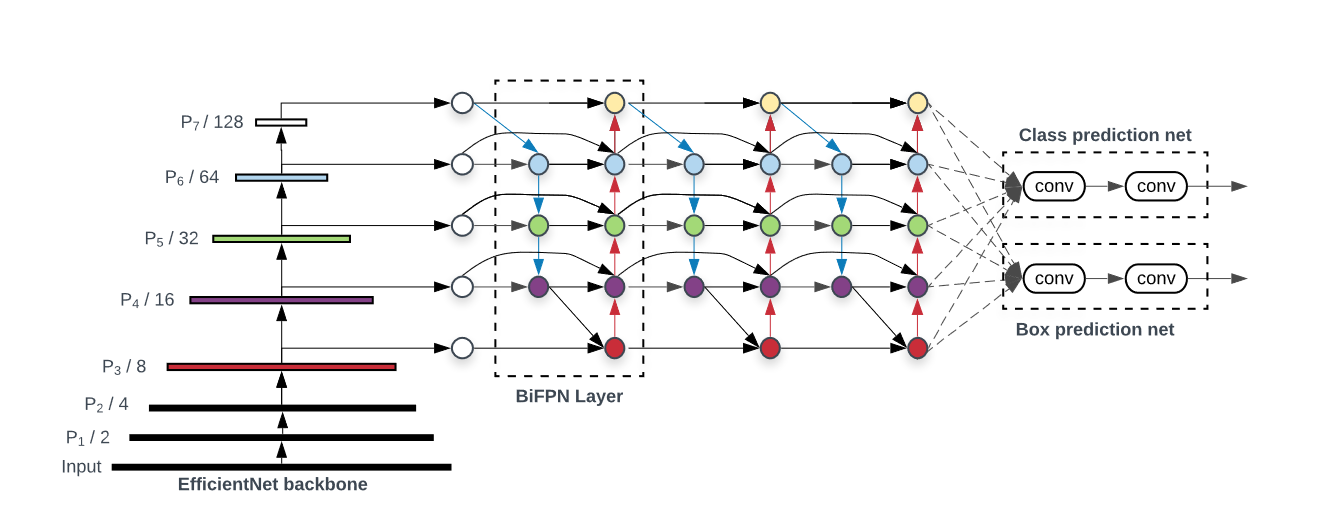
\includegraphics[width=\textwidth]{EfficientDetArchitecture.png}
    \caption{Overview of the EfficientDet architecture. BiFPN layers and subnet layers may be repeated multiple times according to resource constraints.}
    \label{effdet}
\end{figure}

In this chapter we will be providing a brief insight into the EfficientPose pose estimation neural network. EfficientPose was chosen as the starting point for this thesis as it boasts state-of-the-art results while maintaining relative simplicity and low computational costs. It is designed with multi-object estimation in mind, which is especially significant, as other approaches do not scale well with the number of total detections.

\section{Parent Networks}

Similarly to Deep-6DPose (previously mentioned in section \ref*{ss:directestimation}), EfficientPose is an end-to-end direct 6D pose estimation approach that extends the functionality of a 2D network. While Deep-6D extends the segmentation network Mask-R-CNN, EfficientPose extends Google's object classification network EfficientDet\cite{EfficientDet}, which in turn builds on Google's backbone network EfficientNet\cite{EfficientNet}.

Both of these parent networks are based on the concept of scalability: the possibility of increasing network dimensions to achieve better performance in exchange for greater computational cost. These approaches scale using a single hyperparameter, $\phi$. For $\phi = 0$, we have a base network with minimum depth, width and resolution in an optimal ratio. By increasing the value of $\phi$, we can scale up these dimensions while mainining the ratio, thus obtaining better performance than if we had just increased the depth, width or resolution of the network individually.

\begin{figure}[htp]
    \subfloat[EfficientNet: X values are the number of parameters used in the network, Y values are the percentage of correct answers on the Imagenet dataset\cite{imagenet}.]{%
    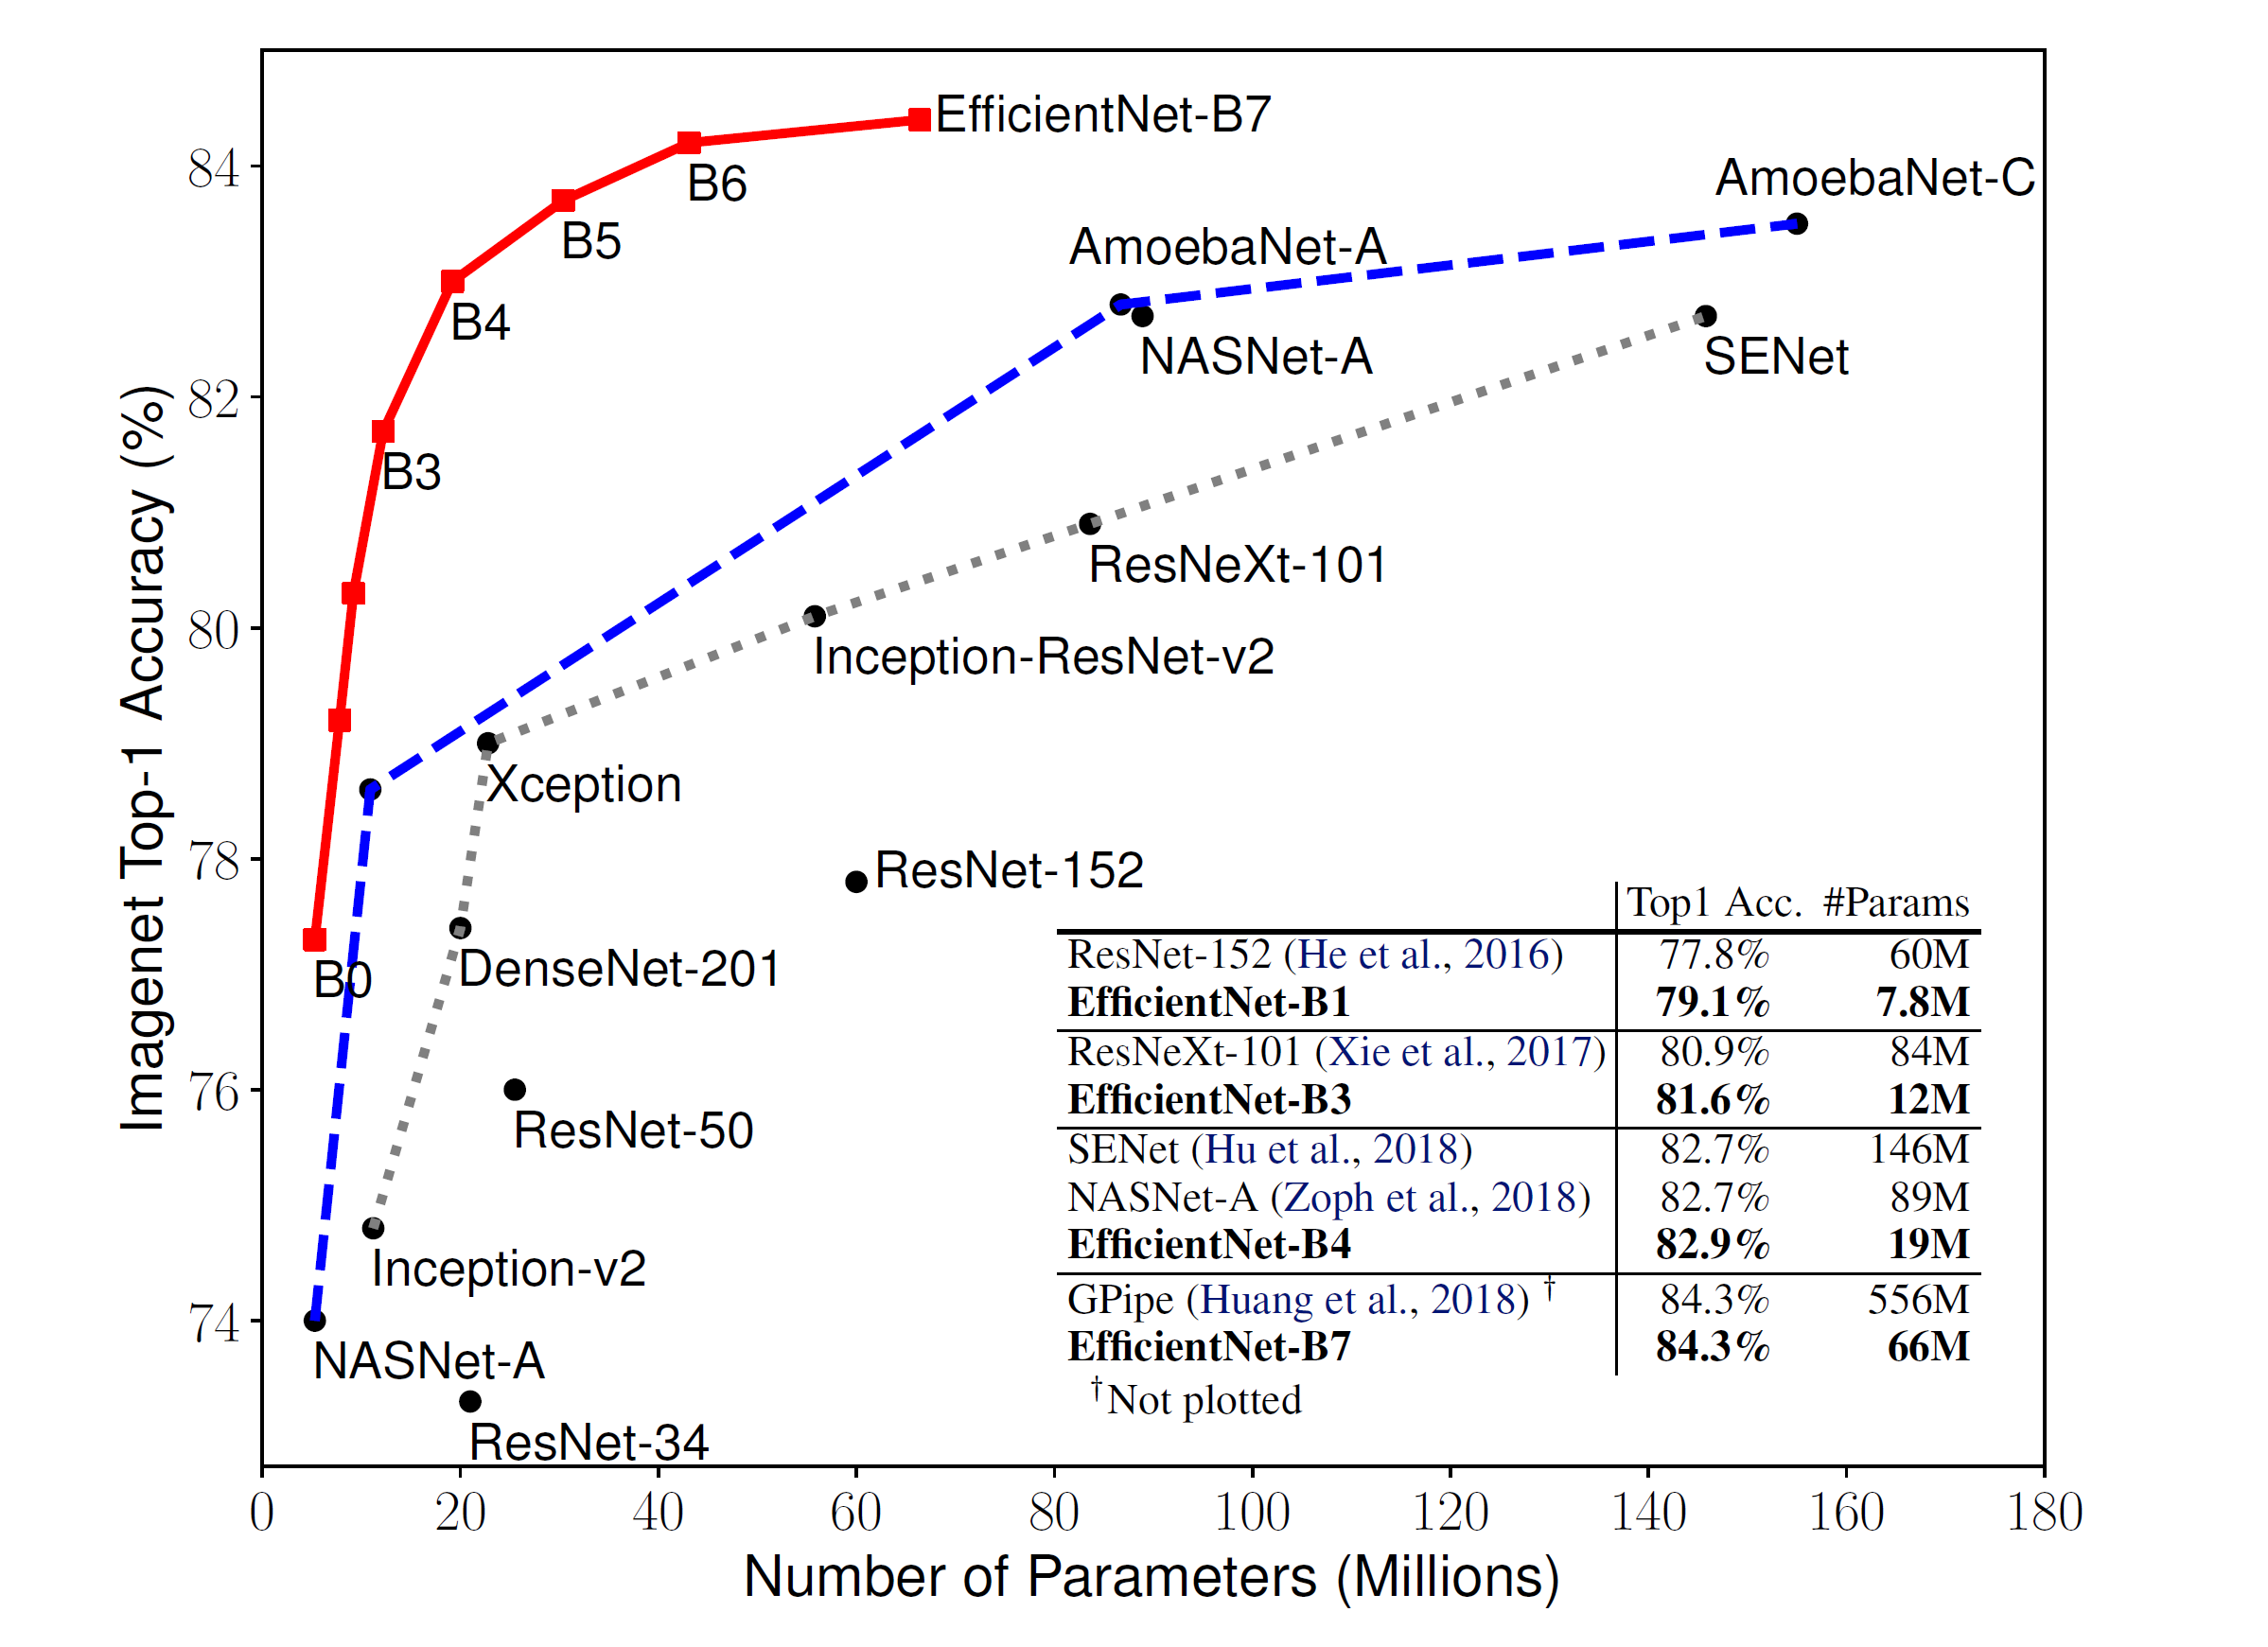
\includegraphics[width=0.7\textwidth]{EfficientNetPerformance.png}
    \label{fig:effNetPerformance}}
    
    \subfloat[EfficientDet: X values are the number of Floating Point Operations per second (FLOPs), Y values are the Average Precision (AP) tested on the Microsoft Commmon Objects in Context dataset\cite{cocodataset}.]{%
    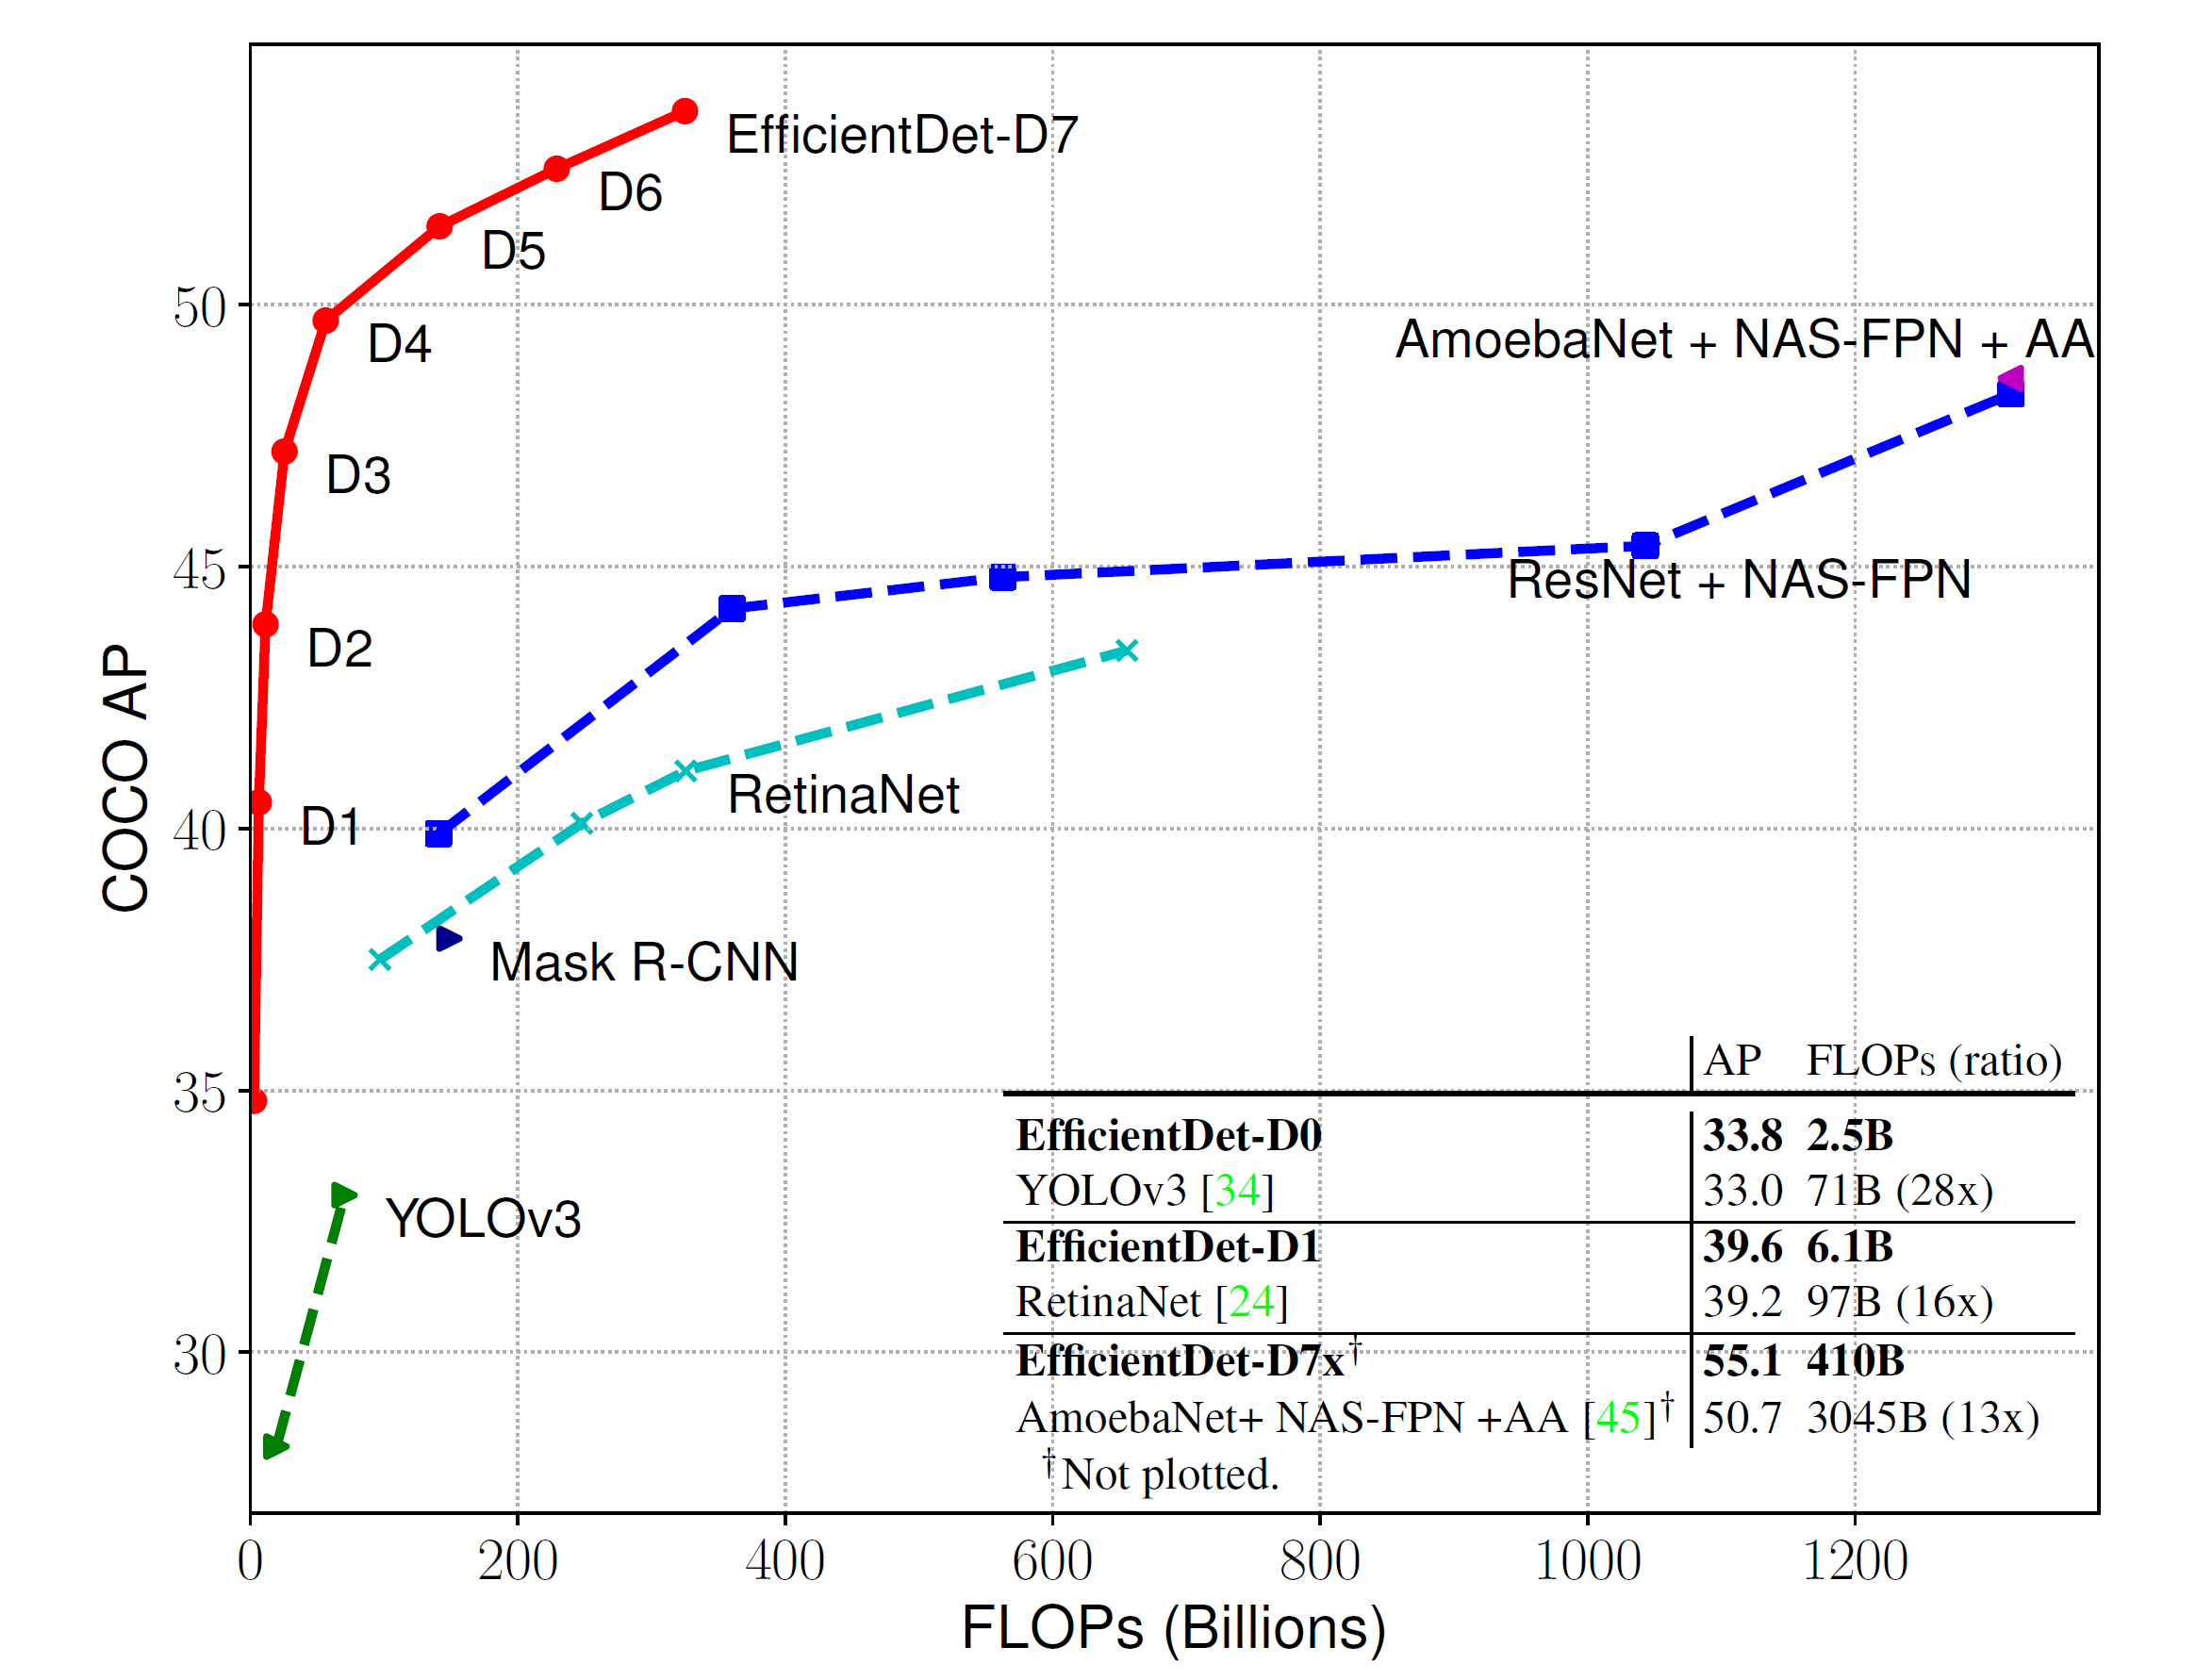
\includegraphics[width=0.7\textwidth]{EfficientDetPerformance.png}
    \label{fig:effDetPerformance}}

    \caption{Performance of the EfficientNet and EfficientDet families compared to other approaches.}
\end{figure}

The backbone of this approach is EfficientNet: a network, or more precisely a family of networks, that was designed using Network Architecture Search (NAS, \cite{NAS}) to provide an optimal ratio of depth, width and resolution. This allows it to obtain a performance that is similar or better than other backbone networks while requiring much fewer parameters, thus greatly lowering computational costs.

EfficientDet then expands on EfficientNet by adding a Feature Pyramid Network (FPNm \cite{FPN}). These networks perform multi-scale feature fusion, combining data from low-resolution, semantically strong layers with data from high-resolution, semantically weak layers. In particular, EfficientDet uses a new form of bi-directional feature pyramids, providing multiple top-down and bottom-up paths with learnable weights. The outputs of this feature network are then fed into multiple subnetworks that use them to perform single tasks, such as object class and 2-D bounding box estimations.

One advantage EfficientDet has over previous 2-D object detectors is that it is single-shot: while other methods require an intermediate region proposal step, EfficientDet performs inference directly on the input image. This means that it requires a significantly lower computational costs, while maintaining state-of-the-art performance.

\section{Methodology}

EfficientPose expands on EfficientDet's architecture with the addition of two additional subnets. These predict translation and rotation for each object class. Since these networks are relatively small, the additional computational costs are minimal.

The rotation network outputs a vector $R \in \mathbb{R}^3$ containing a minimal representation of the rotation in Rodrigues angles, and then employs an additional iterative refinement strategy similar to what is seen in other pose refinement methods. Both the network size and the number of iterations are controlled by the hyperparameter $\phi$.

The translation network instead splits the task of predicting the position $p=[x, y, z]^T$ of the object into separate predictions of the 2D center $c = [c_x, c_y]^T$ and of the depth $z$, similarly to what is done in other direct estimation networks such as PoseCNN \cite{PoseCNN}. The final position $p$ can be computed using the camera intrinsic parameters by inverting the relationship:

\begin{equation}
    \begin{bmatrix}
        c_x\\c_y\\1
    \end{bmatrix}
    = \frac{1}{z}
    \begin{bmatrix}
        f_x & 0 & p_x \\
        0 & f_y & p_y \\
        0 & 0 & 1 
    \end{bmatrix}
    \begin{bmatrix}
        x\\y\\z
    \end{bmatrix}
\end{equation}

...where $f_x, f_y$ are the focal lengths and $(p_x, p_y)$ is the principal point. Thus we obtain:

\begin{equation}
    \begin{bmatrix}
        x\\y\\z
    \end{bmatrix}
    =z
    \begin{bmatrix}
        \frac{1}{f_x} & 0 & \frac{p_x}{f_x} \\
        0 & \frac{1}{f_y} & \frac{p_y}{f_y} \\
        0 & 0 & 1 \\
    \end{bmatrix}
    \begin{bmatrix}
        c_x\\c_y\\1
    \end{bmatrix}
\end{equation}

This also means that EfficientPose is trained on a single set of camera parameters, since the estimation of the depth would be thrown off by changes in the focal distance.

An advantage of EfficientPose's approach is that multiple class, box, rotation and translation networks for different object instances can share the same backbone and feature network. This minimizes additional computation costs for multi-object pose estimation and training, with the downside of losing accuracy compared to a network trained on a single object. 

\section{Performance}

EfficientPose is trained and evaluated on the LINEMOD and Occulsion-LINEMOD datasets, which are standard benchmarks for pose estimation methods.

For single-object estimation on LINEMOD, EfficientPose obtains 97.35\% ADD, placing it at the very top of the state-of-the-art, while for multi-object-estimation on Occlusion-LINEMOD, it obtains 79.04\% ADD with $\phi=0$ and 83.90\% ADD with $\phi=3$.

Also noticeable is the computational performance: while running on an Nvidia RTX 2080 Ti graphics card, with $\phi=0$ it maintained 27.45 FPS for single-object estimation and 26.22 FPS for multi-object estimation.
